%!TEX root = ../main.tex
%%%%%%%%%%%%%%%%%%%%%%%%%%%%%%%%%%
% Links: https://www.geeksforgeeks.org/sort-array-wave-form-2/
%
% Difficulty: Medium Companies: 
%%%%%%%%%%%%%%%%%%%%%%%%%%%%%%%%%%

\chapter{Wave Array}
\label{ch:wave_array}
\section*{Introduction}
We are used to talking about sorting in terms of arranging items in either ascending or descending order. But in general, sorting is the process of arranging items systematically according to a criterion that can be purely arbitrary.

The problem discussed in this lesson is about writing an algorithm for sorting the items of a collection in a rather unusual and peculiar way where the goal is to place elements at even indices such that they all are surrounded by either greater or smaller elements. For instance the collection: $\{1,3,-1,3,2,4\}$ is properly sorted while $\{1,3,-1,1,2,4\}$ is not.

This question has been asked at companies like \textit{Adobe}, and \textit{Google}, mostly during the firsts on-site interview stages as
it is not considered to be a very hard one and you can solve it by writing just a handful of lines.
In fact, provided you come up with the right idea and make no implementation mistakes this problem can be cleared rather quickly. It has, however, proven to be challenging for many, especially in getting it right the first time, and we advise you to spend some time after you have a working draft of the solution to make sure the code is behaving as expected especially on corner cases.






\section{Problem statement}
\begin{exercise}
Given an array $A$ of $n$ integers, arrange the numbers in a wave-like fashion. A valid wave array $X$ has its elements arranged in one of the two following ways:
	\begin{enumerate}
		\item  $x_0 \geq x_1 \leq x_2 \geq x_3 \leq  x_5 \geq \ldots$ where $x_{2i-1} \geq x_{2i} \leq x_{2i+1}$
		\item  $x_1 \leq x_2 \geq x_3 \leq x_4 \geq x_5 \leq \ldots$ where $x_{2i-1} \leq x_{2i} \geq x_{2i+1}$
	\end{enumerate}


	\begin{example}
		\hfill \\
		\label{ex:wave_array:example1}
		Given $A= \{10, 5, 6, 3, 2, 20, 100, 80\}$ the followings are all valid output:
		\begin{itemize}
			\item  \{20, 5, 10, 2, 80, 6, 100, 3\}
			\item  \{10, 5, 6, 2, 20, 3, 100, 80\}
		\end{itemize}
	\end{example}

	\begin{example}
		\hfill \\
		\label{ex:wave_array:example2}
		Given $A= \{20, 10, 8, 6, 4, 2\}$ the followings are all valid output:
		\begin{itemize}
			\item \{20, 8, 10, 4, 6, 2\}
			\item  \{10, 8, 20, 2, 6, 4\}
		\end{itemize}
		
	\end{example}

	\begin{example}
		\hfill \\
		\label{ex:wave_array:example3}
		Given $A= \{10,9,8,7,6,5,4,3,2,1\}$ the following is a output: $\{10, 8, 9, 6, 7, 4, 5, 2, 3, 0,
		1 \}$
		
	\end{example}
\end{exercise}

\begin{figure}
	\centering
	\begin{subfigure}[t]{0.80\textwidth}
		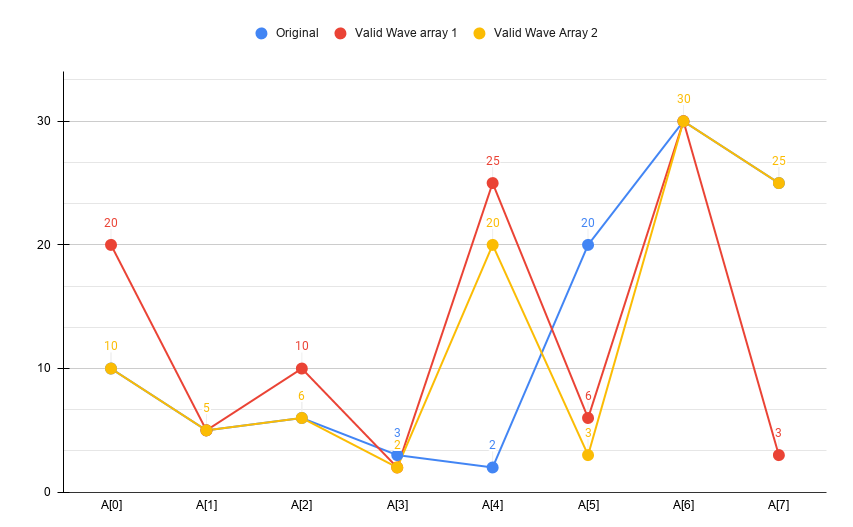
\includegraphics[width=1\linewidth]{sources/wave_array/images/example1.png}
		\caption{Input and solutions for Example \ref{ex:wave_array:example1}.}
		\label{fig:dice_rolls:12faces_dice}
	 \end{subfigure}
	\hfill
	\begin{subfigure}[t]{0.80\textwidth}
		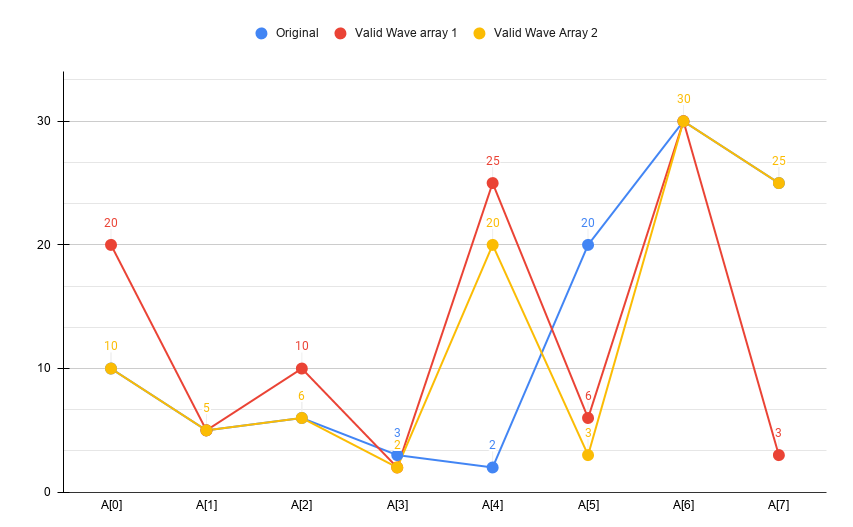
\includegraphics[width=1\linewidth]{sources/wave_array/images/example1.png}
		\caption{Input and solutions for Example \ref{ex:wave_array:example2}.}
		\label{fig:dice_rolls:6faces_dice}
	 \end{subfigure}
	 \hfill
	 \begin{subfigure}[t]{0.80\textwidth}
		 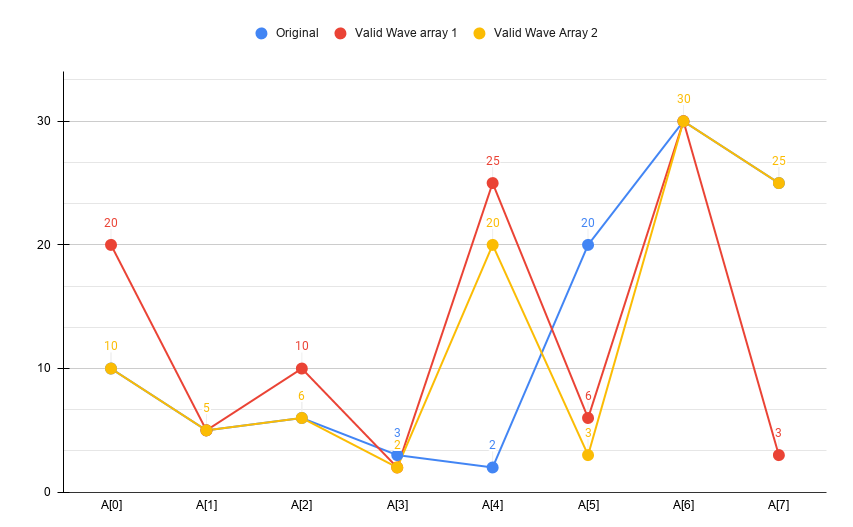
\includegraphics[width=1\linewidth]{sources/wave_array/images/example1.png}
		 \caption{Input and solutions for Example \ref{ex:wave_array:example3}.}
		 \label{fig:dice_rolls:20faces_dice}
	  \end{subfigure}
\end{figure}


\section{Clarification Questions}

\begin{QandA}
	\item Does the array $A$ only contain positive numbers?
	\begin{answered}
		\textit{No, the input numbers can be positive or negative.}
	\end{answered}
	\item Are duplicates in $A$ allowed?
	\begin{answered}
		\textit{Yes, duplicates might be present.}
	\end{answered}
	\item Do the numbers in $A$ lie in a given particular range? If yes which one?
	\begin{answered}
		\textit{No; no assumptions can be made on the values in $A$.}
	\end{answered}
\end{QandA}

\section{Discussion}
\label{wave_array:sec:discussion}
The challenge confronting us is about the creation of an entirely new array $X$ (we, therefore, know from the very beginning we must make a copy of $A$ at some point) that contains the same elements in $A$, arranged in a form that reminds a wave. 
An array of this type has its elements arranged so that they produce a zig-zig-like pattern when plotted on a graph. 

Sequences of numbers of this type can be described as having the property that all of their elements located at even indices are \textbf{all} either 
\textit{local}  \textbf{minima} or  \textbf{maxima}\footnote{An element is a local minimum/maximum if it is lower/higher than its two immediate neighbors.}. 
Identifying a local minimum/maximum is easy but, it is only helpful when we want to test whether a sequence is a valid wave array.

\subsection{Brute-force}
\label{wave_array:sec:bruteforce}
One way to attack this problem is by enumerating every possible arrangement of the elements of $A$ and apply the criteria of wave-array validity discussed above to find a solution. 

We can enumerate all permutations of an array quite easily by using a function like \inline{std::next_permutation](Iterator first, Iterator last)} which 
> Rearranges the elements in the range [first,last) into the next lexicographically greater permutation.

This idea is implemented in Listing \ref{list:wave_array_linear_bruteforce}.

\lstinputlisting[language=c++, caption=Brute-force time solution to the wave array problem.,label=list:wave_array_linear_bruteforce]{sources/wave_array/wave_array_solution3.cpp}


\subsection{Sorting solution}
\label{wave_array:sec:sorting}

As per all array problems, the first question that should come to mind is: \textit{does sorting the elements (we are referring here to a canonical sorting in increasing order) changes the difficulty of the problem?} Incrementally sorted sequences are easy to reason about as they provide strong and clear guarantees on how elements relate to each. Most importantly the same problem is very often a lot easier to solve on a sorted collection than on an unsorted one.
 
If we apply the wave-array validity criterion (discussed above on local minima/maxima) on a sorted array $S=\{s_0 \leq s_1 \leq \ldots \leq s_{n-1}\}$ we notice that $S$ fails the test as there is only one local minimum and local maximum i.e. $s_0$ and $s_{n-1}$ (which also happen to be the global minimum and maximum).

But how $S$ changes if every
element that is located at an even indix is swapped with its subsequent neighbor? When every elements at indices $2i$ and $2i+1$ ($i=0,1,\ldots$) are swapped, then:
$S=\{s_1
\geq s_0 \leq s_3 \geq s_2 \leq s_5 \geq s_4 \leq s_7  \geq \ldots\}$ which is now in better shape to pass the wave-array validity test as now every element at even index is surrounded by smaller (or equal) elements. 

Notice that the elements of $S$ have been shuffled around and that now the element $a_i$ is not located at index $i$ anymore (contrary to how it was originally).
We can see that $a_3$ is now located at index $2$ and it is surrounded by $a_0$ and $a_2$ which are both smaller or equal to $a_3$.
Similarly $a_5$ is now placed at index $4$ and it is surrounded by the elements $a_2$ and $a_4$, both known to be smaller or equal than $a_5$.

We can
use this observation to solve this problem efficiently and elegantly as shown in  Listing \ref{list:wave_array_sorting}.

\lstinputlisting[language=c++, caption=Solution to the wave array problem using sorting.,label=list:wave_array_sorting]{sources/wave_array/wave_array_solution1.cpp}

The code above works by creating a copy of the input array $A$ named $B$, which is subsequently sorted. The code then proceeds in swapping every element located at an even location with the element after it. You can see the \inline{swap} operation is applied to the iterators \inline{it} and \inline{it+1} and that at the end of each iteration \inline{it} is incremented by $2$. This, together with the fact \inline{it} initially pointer to the first even element  at location $0$, effectively means that only pairs of items at indices of the form $(2i, 2i+1)$ are swapped.

The code above is considered good  as its time and space complexity are $O(nlog(n))$
and $O(n)$, respectively.

In some cases, the interviewer might ask you to return, among all possible valid arrangments, the one being the lexicographically minimum. If it is the case the solution proposed below won't
work and it should not be attempted.


\subsection{Linear time solution}

Despite the solution using sorting presented in Section \ref{wave_array:sec:sorting} is already good enough to
possibly clear the interview, there exists a solution that works in linear time and that is as easy to
implement and explain. The core idea is always the same: elements at even index should always be
greater (or smaller, equivalently) than their adjacents neighbors. Only this time we will enforce it in a single pass on the array, by
swapping elements at even indices with their direct neighbors (to the left and to the right) if they happen to be smaller in such a way that the largest element among  $x_{2i-1},x_{2i},x_{2i+1}$ always end up going to the location $2i$.

We can do that by iterating over all even indices and performing the following operations:
\begin{enumerate}
	\item if the current element $a_{2i}$ is smaller than the element $a_{2i-1}$ then swap them. 
	\item if the current element $a_{2i}$ (possibly newly assigned from the previous step) is smaller than the element $a_{2i+1}$ then swap them.
\end{enumerate}

At this point we have effectively placed the largest among $x_{2i-1},x_{2i},x_{2i+1}$ at the location $2i$ and we can proceed to the next even element $a_{2(i+1)}$. 

See Listing \ref{list:wave_array_linear} for a possible implementation of this idea.

\lstinputlisting[language=c++, caption=Linear time solution to the wave array problem.,label=list:wave_array_linear]{sources/wave_array/wave_array_solution2.cpp}

Notice that the code above performs some checks on the corner elements so that we do not perform out-of-bound accesses.

\textbf{This solution is optimal as it runs in $o(n)$ space and time.} 

Like the solution using sorting, it does not work when the lexicographical minimum arrangement should be returned.


